\documentclass[12pt]{article}
\usepackage[margin=1in]{geometry}                % See geometry.pdf to learn the layout options. There are lots.
\geometry{letterpaper}                   % ... or a4paper or a5paper or ... 
%\geometry{landscape}                % Activate for for rotated page geometry
\usepackage[parfill]{parskip}    % Activate to begin paragraphs with an empty line rather than an indent

%%%%%%%%%%%%%%%%%%%%
\newcommand{\hide}[1]{}



\usepackage{natbib}
\usepackage{xcolor}
\usepackage{url}
\usepackage{hyperref}
\usepackage{mathtools}
\usepackage[utf8]{inputenc}
\usepackage{float}
\usepackage{listings}
\usepackage{xcolor}
\usepackage{seqsplit}
\usepackage{verbatim}


\hide{
\usepackage{amscd}
\usepackage{amsfonts}
\usepackage{amsmath}
\usepackage{amssymb}
\usepackage{amsthm}
\usepackage{cases}		 
\usepackage{cutwin}
\usepackage{enumerate}
\usepackage{enumitem}
\usepackage{epstopdf}
\usepackage{graphicx}
\usepackage{ifthen}
\usepackage{lipsum}
\usepackage{mathrsfs}	
\usepackage{multimedia}
\usepackage{wrapfig}
}
\bibliographystyle{humanbio}


\usepackage[utf8]{inputenc}

\newcommand{\itemlist}[1]{\begin{itemize}#1\end{itemize}}
\newcommand{\enumlist}[1]{\begin{enumerate}#1\end{enumerate}}
\newcommand{\desclist}[1]{\begin{description}#1\end{description}}
\newcommand\tab[1][0.5cm]{\hspace*{#1}}

\newcommand{\Answer}[1]{\begin{quote}{\color{blue}#1}\end{quote}}
\newcommand{\AND}{\wedge}
\newcommand{\OR}{\vee}
\newcommand{\ra}{\rightarrow}
\newcommand{\lra}{\leftrightarrow}

\title {{\bf ECE 471 Lab 5} \\
\large{Packet Sniffing and Spoofing Lab / ARP Cache Poisoning Attack Lab
}}

\author{Mitchell Dzurick}
\date{4/15/2020}
\begin{document}

\maketitle
\textbf{Github with all documentation - \url{https://www.github.com/mitchdz/ECE471}}
\tableofcontents 
\clearpage



\section{Packet Sniffing and Spoofing Lab}

\subsection{Task 1.1: Sniffing Packets}
\subsubsection{Task 1.1A}
Wireshark is the most popular sniffing tool, and it is easy to use. We will use it throughout the entire lab.
However, it is difficult to use Wireshark as a building block to construct other tools. We will use Scapy
for that purpose. The objective of this task is to learn how to use Scapy to do packet sniffing in Python
programs. A sample code is provided in the following:
\begin{verbatim}
#!/usr/bin/python
from scapy.all import *

def print_pkt(pkt):
    pkt.show()

pkt = sniff(filter=’icmp’,prn=print_pkt)

if __name__ == "__main__":
    # execute only if run as a script
    print_pkt(pkt)

\end{verbatim}

This code is placed into a file named sniffing.py and made executable with the following command

\begin{verbatim}
$ sudo chown +x sniffing.py
\end{verbatim}
The code can then be ran with the following command
\begin{verbatim}
$ ./sniffing.py
\end{verbatim}

The output after running as root is as follows:
\begin{figure}[H]
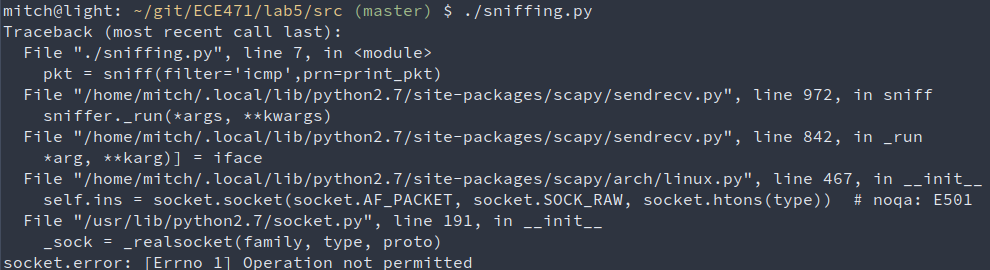
\includegraphics[scale=0.45]{images/p1t1_1.png}
\caption{Running the sniffing program without root}
\label{fig:p1t1_1}
\end{figure}

Looks like we need to utilize root to be able to run this script!

After running the script as root, nothing gets shown because there has been no packets sent yet.

\subsubsection{Task 1.1b}
\tab Usually, when we sniff packets, we are only interested certain types of packets. We can do
that by setting filters in sniffing. Scapy’s filter use the BPF (Berkeley Packet Filter) syntax; you can find the
BPF manual from the Internet. Please set the following filters and demonstrate your sniffer program again
(each filter should be set separately):
\begin{enumerate}
	\item Capture only the ICMP packet
	\item Capture any TCP packet that comes from a particular IP and with a destination port number 23.
	\item Capture packets comes from or to go to a particular subnet. You can pick any subnet, such as
	128.230.0.0/16; you should not pick the subnet that your VM is attached to.
\end{enumerate}

1. pkt = sniff(filter="icmp")

To only pull icmp packets, you can use the filter option to force only icmp packets to show up.

2. pkt = sniff(filter="tcp and port 23 and host 66.35.250.151")

To pull up only tcp packets on a certain port from a certain host, the preceding filter can be applied. To chain together multiple filters, you can simply put the keyword `and` between the filters. `tcp`, `port 23`, `host 66.35.250.151`.

3. pkt = sniff(filter="host 128.230.0.0/16")

To gather packets on a subnet, the above filter is applied!



\subsection{Task 1.2: Spoofing ICMP Packets}

As a packet spoofing tool, Scapy allows us to set the fields of IP packets to arbitrary values. The objective
of this task is to spoof IP packets with an arbitrary source IP address. We will spoof ICMP echo request
packets, and send them to another VM on the same network. We will use Wireshark to observe whether our
request will be accepted by the receiver. If it is accepted, an echo reply packet will be sent to the spoofed IP
address. The following code shows an example of how to spoof an ICMP packets.

\begin{verbatim}
>>> from scapy.all import
>>> a = IP()
>>> a.dst = ’10.0.2.3’
>>> b = ICMP()
>>> p = a/b
>>> send(p)
.
Sent 1 packets.
\end{verbatim}
In the code above, Line À creates an IP object from the IP class; a class attribute is defined for each IP
header field. We can use ls(a) or ls(IP) to see all the attribute names/values. We can also use a.show()
and IP.show() to do the same. Line Á shows how to set the destination IP address field. If a field is not set,
a default value will be used.

Line  creates an ICMP object. The default type is echo request. In Line Ã, we stack a and b together
to form a new object. The / operator is overloaded by the IP class, so it no longer represents division;
instead, it means adding b as the payload field of a and modifying the fields of a accordingly. As a result,
we get a new object that represent an ICMP packet. We can now send out this packet using send() in
Line Ä. Please make any necessary change to the sample code, and then demonstrate that you can spoof an
ICMP echo request packet with an arbitrary source IP address.


And here is the results of sniffing the packet using the program from Task1.1a.
\begin{verbatim}
###[ Ethernet ]###
dst       = 3c:37:86:f2:c4:56
src       = d0:ab:d5:bb:40:f9
type      = IPv4
###[ IP ]###
version   = 4
ihl       = 5
tos       = 0x0
len       = 28
id        = 1
flags     =
frag      = 0
ttl       = 64
proto     = icmp
chksum    = 0xad33
src       = 192.168.1.2
dst       = 10.0.2.3
\options   \
###[ ICMP ]###
type      = echo-request
code      = 0
chksum    = 0xf7ff
id        = 0x0
seq       = 0x0
\end{verbatim}

This shows that we can utilize scapy to do exactly what is says it should do.




\subsection{Task 1.4: Sniffing and-then Spoofing (Extra Credit)}
In this task, you will combine the sniffing and spoofing techniques to implement the following sniff-and-
then-spoof program. You need two VMs on the same LAN. From VM A, you ping an IP X. This will
generate an ICMP echo request packet. If X is alive, the ping program will receive an echo reply, and
print out the response. Your sniff-and-then-spoof program runs on VM B, which monitors the LAN through
packet sniffing. Whenever it sees an ICMP echo request, regardless of what the target IP address is, your
program should immediately send out an echo reply using the packet spoofing technique. Therefore, regard-
less of whether machine X is alive or not, the ping program will always receive a reply, indicating that X
is alive. You need to use Scapy to do this task. In your report, you need to provide evidence to demonstrate
that your technique works.
\subsubsection{Task 1.4: Solution}
To execute this task, two virtual machines need to be created. The following script is used with a Vagrantfile in order to populate virtual machines for us.

The following Vagrantfile is used to spawn two virtual machines, "a" and "b"


\begin{verbatim}
# -*- mode: ruby -*-
# vi: set ft=ruby :

# Vagrant multi-machine sample setup

$script = <<SCRIPT
# download required packages
apt-get -y update
apt-get -y install git vim python-scapy
SCRIPT

BOX_IMAGE="hashicorp/precise64"


Vagrant.configure("2") do |config|

  config.vm.define :a do |a|
    a.vm.box = BOX_IMAGE
    a.vm.network :private_network, ip: "10.0.0.11"
    a.vm.hostname = "a"
  end

  config.vm.define :b do |b|
    b.vm.box = BOX_IMAGE
    b.vm.network :private_network, ip: "10.0.0.12"
    b.vm.hostname = "b"
    b.vm.provider :virtualbox do |vb|
      # more RAM
      vb.customize ["modifyvm", :id, "--memory", "4096"]
      # enable promiscuous mode on the public network
      vb.customize ["modifyvm", :id, "--nicpromisc3", "allow-all"]
    end
  end

  config.vm.provision "shell", inline: $script
end
\end{verbatim}

With this file in any directory, run the command `vagrant up` and the machines will be populated. To ssh into machine a, run the command `vagrant ssh a`, for b you will run the command `vagrant ssh b`.

The following commands are shown in machine b.


\begin{verbatim}
vagrant@b:/vagrant/src$ ifconfig | grep "inet addr"
inet addr:10.0.2.15  Bcast:10.0.2.255  Mask:255.255.255.0
inet addr:10.0.0.12  Bcast:10.0.0.255  Mask:255.255.255.0
inet addr:127.0.0.1  Mask:255.0.0.0
vagrant@b:/vagrant/src$ cat spoofing.py
#!/usr/bin/python
from scapy.all import *

def print_pkt(pkt):
pkt.show()
a=IP(dst=pkt[IP].src)/ICMP)
sr1(a)

pkt = sniff(filter='icmp',prn=print_pkt)
vagrant@b:/vagrant/src$
\end{verbatim}

running `sudo python /vagrant/src/spoofing.py` in machine b starts our program. On machine a, we can ping machine b and see normal ICMP response.

\begin{verbatim}
vagrant@a:~$ ping -c 1 10.0.0.12
PING 10.0.0.12 (10.0.0.12) 56(84) bytes of data.
64 bytes from 10.0.0.12: icmp_req=1 ttl=64 time=0.828 ms

--- 10.0.0.12 ping statistics ---
1 packets transmitted, 1 received, 0% packet loss, time 0ms
rtt min/avg/max/mdev = 0.828/0.828/0.828/0.000 ms
\end{verbatim}

However, with our program running in the background (and b running in promiscuous mode), we see the valid response from machines that do not exist.

\begin{verbatim}
vagrant@a:~$ ping -c 1 10.0.0.10
PING 10.0.0.10 (10.0.0.10) 56(84) bytes of data.
64 bytes from 10.0.0.10: icmp_req=1 ttl=64 time=1.54 ms

--- 10.0.0.10 ping statistics ---
1 packets transmitted, 1 received, 0% packet loss, time 0ms
rtt min/avg/max/mdev = 1.547/1.547/1.547/0.000 ms
\end{verbatim}







\section{ARPCache Poisoning Attack Lab}
\subsection{Task 2.1: ARP Cache Poisoning}
The objective of this task is to use packet spoofing to launch an ARP cache poisoning attack on a target,
such that when two victim machines A and B try to communicate with each other, their packets will be
intercepted by the attacker, who can make changes to the packets, and can thus become the man in the
middle between A and B. This is called Man-In-The-Middle (MITM) attack. In this lab, we use ARP cahce
poisoning to conduct an MITM attack. \\
\tab The following code skeleton shows how to construct an ARP packet using Scapy.
\begin{verbatim}
#!/usr/bin/python3
from scapy.all import *
E = Ether()
A = ARP()
pkt = E/A
sendp(pkt)
\end{verbatim}

\tab The above program constructs and sends an ARP packet. Please set necessary attribute names/values to
define your own ARP packet. We can use ls(ARP) to see the attribute names of the ARP class. If a field
is not set, a default value will be used (see the third column of the output):

\begin{verbatim}
>>> from scapy.all import *
>>> ls(ARP)
<data about ARP>
\end{verbatim}
In this task, we have three VMs, A, B, and M. We would like to attack A’s ARP cache, such that the
following results is achieved in A’s ARP cache.

\begin{verbatim}
B’s IP address --> M’s MAC address
\end{verbatim}
There are many ways to conduct ARP cache poisoning attack. Students need to try the following three
methods, and report whether each method works or not.

\begin{itemize}
	\item \textbf{Task 1A} (using ARP request). On host M, construct an ARP request packet and send to host A.
	Check whether M’s MAC address is mapped to B’s IP address in A’s ARP cache.
	\item \textbf{Task 1B} (using ARP reply). On host M, construct an ARP reply packet and send to host A. Check
	whether M’s MAC address is mapped to B’s IP address in A’s ARP cache.
	\item \textbf{Task 1C} (using ARP gratuitous message). On host M, construct an ARP gratuitous packets. ARP
	gratuitous packet is a special ARP request packet. It is used when a host machine needs to update
	outdated information on all the other machine’s ARP cache. The gratuitous ARP packet has the
	following characteristics:
	\begin{itemize} 
		\item The source and destination IP addresses are the same, and they are the IP address of the host
		issuing the gratuitous ARP.
		\item The destination MAC addresses in both ARP header and Ethernet header are the broadcast MAC
		address (ff:ff:ff:ff:ff:ff).
		\item No reply is expected.
		
	\end{itemize}
\end{itemize}


To execute this lab, the following script is used inside a file named `VagrantFile`
\begin{verbatim}
# -*- mode: ruby -*-
# vi: set ft=ruby :

# Vagrant multi-machine sample setup

Vagrant.configure("2") do |config|
  config.vm.define :m do |m|
    m.vm.box = "hashicorp/precise64"
    m.vm.network :private_network, ip: "10.0.0.10"
    m.vm.hostname = "m"
  end

  config.vm.define :a do |a|
     a.vm.box = "hashicorp/precise64"
     a.vm.network :private_network, ip: "10.0.0.11"
     a.vm.hostname = "a"
  end

  config.vm.define :b do |b|
    b.vm.box = "hashicorp/precise64"
    b.vm.network :private_network, ip: "10.0.0.12"
    b.vm.hostname = "b"
  end
end
\end{verbatim}

To populate the virtual machines, run the following command in the directory that the VagrantFile exists in:

\begin{verbatim}
$ vagrant up
\end{verbatim}
This command will provision 3 machines each with host name `m`, `a`, `b`.

You can then ssh into these virtual machines with the following command:
\begin{verbatim}
$ vagrant ssh [m|a|b]
\end{verbatim}
Where you choose whether to ssh into m, a, or b.


\subsubsection{1A}





\subsubsection{1B}
\subsubsection{1C}







\end{document}

